\documentclass[]{book}
\usepackage{lmodern}
\usepackage{amssymb,amsmath}
\usepackage{ifxetex,ifluatex}
\usepackage{fixltx2e} % provides \textsubscript
\ifnum 0\ifxetex 1\fi\ifluatex 1\fi=0 % if pdftex
  \usepackage[T1]{fontenc}
  \usepackage[utf8]{inputenc}
\else % if luatex or xelatex
  \ifxetex
    \usepackage{mathspec}
  \else
    \usepackage{fontspec}
  \fi
  \defaultfontfeatures{Ligatures=TeX,Scale=MatchLowercase}
\fi
% use upquote if available, for straight quotes in verbatim environments
\IfFileExists{upquote.sty}{\usepackage{upquote}}{}
% use microtype if available
\IfFileExists{microtype.sty}{%
\usepackage{microtype}
\UseMicrotypeSet[protrusion]{basicmath} % disable protrusion for tt fonts
}{}
\usepackage{hyperref}
\hypersetup{unicode=true,
            pdftitle={A Compact Guide to Classical Inference},
            pdfauthor={Daniel Kaplan},
            pdfborder={0 0 0},
            breaklinks=true}
\urlstyle{same}  % don't use monospace font for urls
\usepackage{natbib}
\bibliographystyle{apalike}
\usepackage{longtable,booktabs}
\usepackage{graphicx,grffile}
\makeatletter
\def\maxwidth{\ifdim\Gin@nat@width>\linewidth\linewidth\else\Gin@nat@width\fi}
\def\maxheight{\ifdim\Gin@nat@height>\textheight\textheight\else\Gin@nat@height\fi}
\makeatother
% Scale images if necessary, so that they will not overflow the page
% margins by default, and it is still possible to overwrite the defaults
% using explicit options in \includegraphics[width, height, ...]{}
\setkeys{Gin}{width=\maxwidth,height=\maxheight,keepaspectratio}
\usepackage[normalem]{ulem}
% avoid problems with \sout in headers with hyperref:
\pdfstringdefDisableCommands{\renewcommand{\sout}{}}
\IfFileExists{parskip.sty}{%
\usepackage{parskip}
}{% else
\setlength{\parindent}{0pt}
\setlength{\parskip}{6pt plus 2pt minus 1pt}
}
\setlength{\emergencystretch}{3em}  % prevent overfull lines
\providecommand{\tightlist}{%
  \setlength{\itemsep}{0pt}\setlength{\parskip}{0pt}}
\setcounter{secnumdepth}{5}
% Redefines (sub)paragraphs to behave more like sections
\ifx\paragraph\undefined\else
\let\oldparagraph\paragraph
\renewcommand{\paragraph}[1]{\oldparagraph{#1}\mbox{}}
\fi
\ifx\subparagraph\undefined\else
\let\oldsubparagraph\subparagraph
\renewcommand{\subparagraph}[1]{\oldsubparagraph{#1}\mbox{}}
\fi

%%% Use protect on footnotes to avoid problems with footnotes in titles
\let\rmarkdownfootnote\footnote%
\def\footnote{\protect\rmarkdownfootnote}

%%% Change title format to be more compact
\usepackage{titling}

% Create subtitle command for use in maketitle
\providecommand{\subtitle}[1]{
  \posttitle{
    \begin{center}\large#1\end{center}
    }
}

\setlength{\droptitle}{-2em}

  \title{A Compact Guide to Classical Inference}
    \pretitle{\vspace{\droptitle}\centering\huge}
  \posttitle{\par}
    \author{Daniel Kaplan}
    \preauthor{\centering\large\emph}
  \postauthor{\par}
      \predate{\centering\large\emph}
  \postdate{\par}
    \date{2019-11-01}

\usepackage{booktabs}
\usepackage{booktabs}
\usepackage{longtable}
\usepackage{array}
\usepackage{multirow}
\usepackage{wrapfig}
\usepackage{float}
\usepackage{colortbl}
\usepackage{pdflscape}
\usepackage{tabu}
\usepackage{threeparttable}
\usepackage{threeparttablex}
\usepackage[normalem]{ulem}
\usepackage{makecell}
\usepackage{xcolor}

\begin{document}
\maketitle

{
\setcounter{tocdepth}{1}
\tableofcontents
}
\hypertarget{what-is-classical-inference}{%
\chapter{What is classical inference?}\label{what-is-classical-inference}}

Statistical inference is the logic and methods for creating statistical claims that are justified by data. A \emph{statistical claim} is a statement like this: My data show that taking aspirin is associated with a reduction in fever. Or this: My data show that for every year of age, middle-aged runners slow down, on average, by 20-40 seconds per mile.

Statistical inference was invented to guard against spurious claims. For instance, suppose you had these data on age and running times (in minutes) in a 10-mile road race:

\begin{longtable}[]{@{}lll@{}}
\toprule
Person & Age & Running Time\tabularnewline
\midrule
\endhead
John & 48 & 105\tabularnewline
Abigail & 40 & 101\tabularnewline
\bottomrule
\end{longtable}

Just comparing the ages and running times of John and Abigail, you can see that John is 4 minutes (that is, 240 seconds) slower than Abigail in completing the 10 mile run. Their age difference is 8 years. This amounts to and additional 30 seconds of running time per year of age difference. (240 / 8 = 30.) Since you are uncertain -- this is only one race, this is only two people, etc. -- you decide to frame your findings this way: My data show that middle-aged runners slow down by 20-40 seconds/mile for every year additional age. That is a statistical claim.

There are many problems with this statistical claim. First, it's comparing people with more differences than 8 years of age. To judge from the names, John is a man and Abigail a woman. A different statistical statement prompted by the data is that women are faster than men by 30 seconds per mile. Or, it might be that Abigail is an experience runner and John is a formerly lethargic man who has been trying to build up to being able to run 10 miles. (Congratulations, John! A ten-mile time of 105 minutes is a pretty impressive accomplishment.)

Common sense -- and good statistical practice -- tells you to compare like with like. Wouldn't it be better to compare men of different ages who are both running their first 10-mile race? Or, how about looking at Abigail's past records from when she was younger? The failure to do things like this is reason enough to be skeptical about the 20-40 seconds/mile per year claim. But this is a flaw in study design and the collection of data. That is not the kind of flaw that statistical inference deals with.

Statistical inference deals with one, and only one, source of uncertainty: that produced by the size of the sample, in this case 2 people. Again, common sense tells you that two is not a lot of data. So, how much would be enough? 10? 100? 1000? Or, put another way, how should you frame the uncertainty in your claim due to limited data? In the example, the 20-40 seconds/mile per year interval was made up to create an impression of scientific precision. Statistical inference techniques create a meaningful interval that stems from the data itself, rather than the imagination of the researcher.

The need for statistical inference became important when it was realized, around 1900, that there was not yet a reliable way of knowing how much data -- that is, how many rows of data -- is sufficient. The founders of statistical inference found ways to frame the problem in terms of the mathematics of probability, and used algebra and other mathematical techniques to solve the problem. They summarized the process of statistical inference using formulas and tables of probabilities. This is \emph{classical} inference.

Algeba and other mathematical arguments can be difficult and subtle. In the early days of classical inference there were disagreements about what formulas would be best. To develop ideas and confirm that their formulas gave reasonable results, some of the founders of classical inference used \emph{simulations}. One simulation, for instance, involved writing down data for 3000 individual people on index cards, shuffling the cards, then dealing out hands of 4 cards each. With 1000 such events, it was straightforward -- but extremely tedious -- to see what results were likely and which not.

The algebraic techniques were pretty much the only way to conduct statistical inference until the 1970s. Then, as computing became available at research institutions, the simulation technique became easy enough to be practical for routine problems in statistical inference. Simulation on computers became a potential substitute for algebra.

Perhaps many students would agree that anything that reduces the amount of algebra needed to solve a problem is worthwhile. But this is not the fundamental reason why simulation is an important technique. Yes, simulation is easy, but because it's easy it can be applied to situations which were too complicated to handle reliably with algebra, even by the best of mathematicians. The simulation approach to statistical inference has been called \emph{computer-age statistical inference} to distinguish it from \emph{classical statistical inference}.

\hypertarget{and-why-should-i-read-this-book}{%
\section*{\ldots{} and why should I read this book?}\label{and-why-should-i-read-this-book}}
\addcontentsline{toc}{section}{\ldots{} and why should I read this book?}

We live in the computer age, so you might suppose that statistics courses would use computer-age statistical inference. By and large they do not. Why not? There is one good reason and several bad reasons for this. And these reasons -- good and bad -- determine whether you should read this book.

Classical inference is the only way to conduct statistical inference for very small data, say with 10 or fewer rows of data. So if you are working with small data, you need to learn classical inference.

And even if you don't need to work with such small data, there may be reasons for you to learn something about classical inference. One is that, if you are taking an introductory course, chances are a substantial part of the course is about classical inference. This is more or less a ``because I said so'' justification for studying a topic.

Putting aside the matter of small data, instructors use classical inference because that is what they were taught. They don't use simulation for a variety of reasons: they may not know about the computer-age techniques, they may not be comfortable teaching how to use a computer, they may see algebra as prestigious and computing as low-class, they may think their students don't have access to computing (and in some places, this might be right), they may have been forced to use the n\textsuperscript{th} edition of a textbook originally written before computer-age inference was accessible and which continues to use classical inference because it's hard for an instructor to change textbooks.

My personal view is that everyone studying statistics should learn computer-age statistical inference. First, most students find it much easier, so they can spend their mental energy to understand the purpose of statistical inference rather than the mechanics of it. Second, it makes it straightforward to move away from the classical settings (e.g.~the difference in two proportions, straight-line models) and toward settings that are more important today (e.g.~risk ratios, machine learning models). Third, learning to use a computer is itself a valuable objective. In my view, it's only worthwhile to learn classical inference when you are confronted with small-data situations or when your interest in statistics is deep.

But if you \emph{have to} study classical inference, you might as well study it in a concise way. The traditional classical inference curriculum uses a large amount of confusing terminology and splits the subject into several different topics even though they are all very much the same thing. Also, if you are studying statistical inference you are learning how to express uncertainty. Ironically, the textbook description of classical inference involves detailed calculations of great precision. That precision is unjustified. The needless precision is in the textbooks because that's what happens when you translate a real-world problem into deterministic mathematics and because the culture of mathematics education is that of exactitude and proof. Exactitude and proof are valuable things in the proper setting. But in statistical inference, rough answers are good enough. Indeed, the leading professional organization of statisticians, the American Statistical Association, has explicitly called for practitioners of statistical inference to \emph{stop} suggesting that the precision of classical textbook answers is meaningful.

In order to write a compact guide to statistical inference, I've translated the classical texts into a modern statistical language and computer oriented notation. We'll be using models and effect sizes. All the different settings of textbook classical inference can be expressed in the same way, so we'll work with this one way rather than the six or seven found in textbooks. We'll dispense with unnecessary intermediates such as the ``standard error'' and dodge the doubtful digressions into misleading exactitude that unnecessarily increases the difficulty of learning and understanding classical inference.

\hypertarget{data-and-variables}{%
\chapter{Data and variables}\label{data-and-variables}}

\hypertarget{data-frames}{%
\section{Data frames}\label{data-frames}}

Although this book is a guide to classical inference, we will work with data in a contemporary format. The data we use is organized into \emph{data frames}, which are more-or-less spreadsheets. The columns of the data frame are \emph{variables}, the rows of the data frame are \emph{units of observation}.

As an example, consider data collected by Francis Galton, one of the pioneers of statistics. In the 1880s, seeking to understand genetic inheritance from parent to child, Galton visited almost 200 families in London with both parents living and children who had grown up. Galton recorded the height of the mother and father, and the height and sex of each of the adult children. Figure @ref\{fig:galton-raw\} shows part of the data frame.

\begin{table}[t]

\caption{\label{tab:unnamed-chunk-2}Figure 1: The `Galton` data frame containing Galtons measurements of 898 adult children.}
\centering
\begin{tabular}{l|r|r|l|r|r}
\hline
family & father & mother & sex & height & nkids\\
\hline
1 & 78.5 & 67.0 & M & 73.2 & 4\\
\hline
1 & 78.5 & 67.0 & F & 69.2 & 4\\
\hline
1 & 78.5 & 67.0 & F & 69.0 & 4\\
\hline
1 & 78.5 & 67.0 & F & 69.0 & 4\\
\hline
2 & 75.5 & 66.5 & M & 73.5 & 4\\
\hline
2 & 75.5 & 66.5 & M & 72.5 & 4\\
\hline
2 & 75.5 & 66.5 & F & 65.5 & 4\\
\hline
2 & 75.5 & 66.5 & F & 65.5 & 4\\
\hline
3 & 75.0 & 64.0 & M & 71.0 & 2\\
\hline
3 & 75.0 & 64.0 & F & 68.0 & 2\\
\hline
\multicolumn{6}{l}{... and so on for 898 rows altogether.}\\
\end{tabular}
\end{table}

Each row corresponds to a unit of analysis, in this case, a person. The first row is a 6 foot 1.2 inch man, in a family with 4 kids altogether. Looking at the next three rows, you see his three sisters, who are quite tall for the time (5 foot 9 inches) but not as tall as their parents. Their mother was a bit shorter (5 foot 7) and their father was very tall even by today's standards: 6 feet 6.5 inches.

The family is designated with a number. So all four of the first rows are kids in family one, while rows 5 and 6 come from family two.

Most of the variables are \emph{numeric}, as appropriate for height and the number of kids. One variable, \texttt{sex}, has values that are labels, M and F here, standing for male and female. Such variables are called \emph{categorical}; the possible labels are the \emph{levels} of the variable. In this book, categorical variables with \emph{two levels} will play a very important role, but certainly there are categorical variables with more than two levels, as we shall see.

The \texttt{family} variable has been encoded as a number, but it is not really numerical. For instance, with numbers, 2 is half way between 1 and 3. But family 2 is not ``between'' families 1 and 2 in any genuinely numerical sense.

\hypertarget{tabulations}{%
\section{Tabulations}\label{tabulations}}

Historically, when data was shared by printing it and when calculations were tedious, data would often be presented as \emph{tabulations}. For instance, one of the very early (Punnet 1905, p.~93) investigations of cross-linkage in genetics examined 799 sweet pea plants, recording the color of the flower and whether the pollen was round or elongated.

\begin{figure}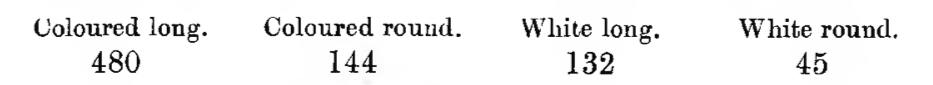
\includegraphics[width=0.8\linewidth]{images/Punnet-page-93} \caption{Figure 3: Genetics data from 1905}\label{fig:punnet-93}
\end{figure}

This style of presentation is perfectly understandable, but it is not in the modern format for data. As a data table, this would look like:

\begin{table}[t]

\caption{\label{tab:punnet-raw}Figure 4: Punnet's data in a contemporary format}
\centering
\begin{tabular}{l|l|l}
\hline
ID & flower\_color & pollen\_shape\\
\hline
SP2760 & other & long\\
\hline
SP5930 & other & round\\
\hline
SP7510 & white & long\\
\hline
SP5820 & other & round\\
\hline
SP2070 & other & long\\
\hline
SP5350 & other & round\\
\hline
\multicolumn{3}{l}{... and so on for 801 rows altogether.}\\
\end{tabular}
\end{table}

Punnett from Bateson, W., et al.~Experimental studies in the physiology of heredity. Reports to the Evolution Committee of the Royal Society 2, 1--55, 80--99 (1905) p.~93.

You may well wonder what benefit there is to working with an 801-row data frame rather than the simple tabulation in the original publication. First, giving the variables names allows us to distinguish between the variable being measured and the level of the measurement. Second, the table makes clear that both variables \texttt{flower\_color} and \texttt{pollen\_shape} are categorical. Third, suppose there was some other aspect being recorded about the plants, for instance the plant's height or how much water the plant was given or the name of the technician who recorded the data. Using a data frame, these new variables can easily be added as additional columns. There's no space in the tabulation for these additional measurements.

A fourth reason to prefer the data-frame format for the genetics data is subtle. Most often, you will be using software to analyze data. Storing data in a consistent way -- data frames -- makes it much easier to use standard software than if the data are stored in a (pointless) variety of formats. Even in classical days, the variety of formats used to store data resulted in the creation of ``new'' statistical methods that were set up to deal with the special format in which data was presented.

\hypertarget{quantitative-and-categorical}{%
\section{Quantitative and categorical}\label{quantitative-and-categorical}}

\hypertarget{indicator-variables}{%
\section{Indicator variables}\label{indicator-variables}}

For a categorical variable: is it level X?

\hypertarget{response-and-explanatory-variables}{%
\section{Response and explanatory variables}\label{response-and-explanatory-variables}}

\hypertarget{other-data-sets.-just-for-my-notes.}{%
\subsubsection*{OTHER DATA SETS. Just for my notes.}\label{other-data-sets.-just-for-my-notes.}}
\addcontentsline{toc}{subsubsection}{OTHER DATA SETS. Just for my notes.}

\hypertarget{gosset}{%
\subsubsection{Gosset}\label{gosset}}

\texttt{datasets::crimtab}, maybe use dichotimization of data to illustrate other points.

\hypertarget{cushny-and-peeples}{%
\subsubsection{Cushny and Peeples}\label{cushny-and-peeples}}

\texttt{psych::cushny}

Look at the fractional change in sleep time from control, not the time difference. (There are a lot of people getting very little sleep!)

\hypertarget{hooker-and-yule}{%
\subsubsection{Hooker and Yule}\label{hooker-and-yule}}

Note on Estimating the Relative Influence of Two Variables upon a Third
Author(s): R. H. Hooker and G. U. Yule
Source: Journal of the Royal Statistical Society, Vol. 69, No.~1 (Mar., 1906), pp.~197-200 Published by: Wiley for the Royal Statistical Society

\begin{figure}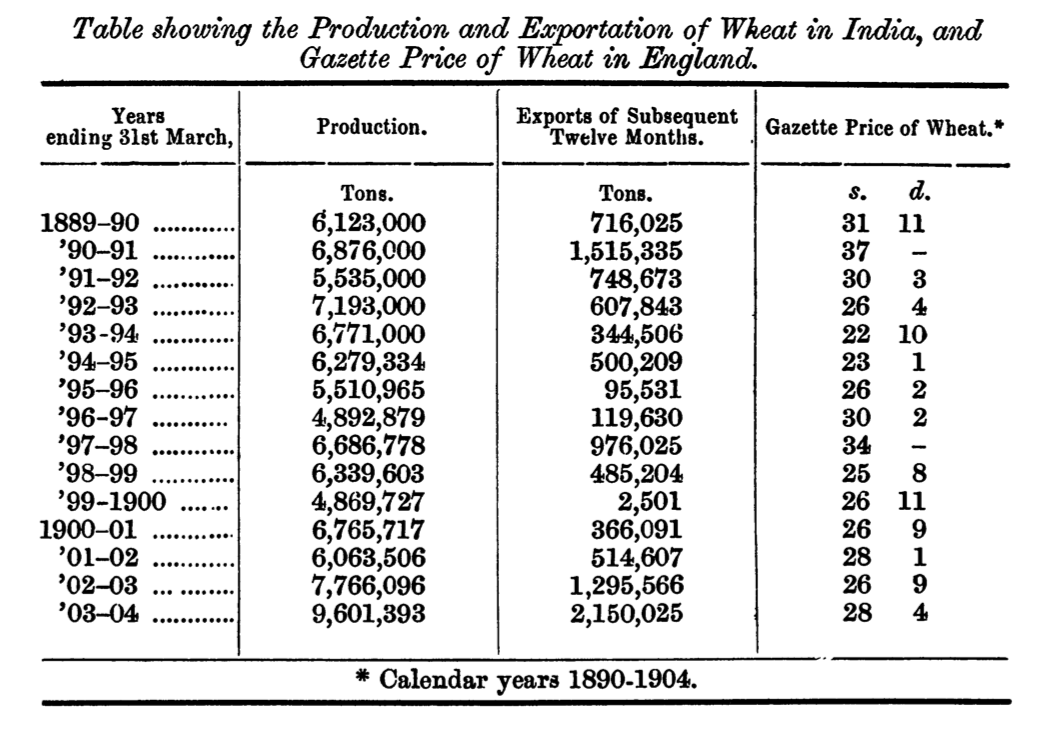
\includegraphics[width=0.8\linewidth]{images/india-exports-yule} \caption{Figure 2: Wheat production and export in India, and prices in Britain}\label{yule-exports}
\end{figure}

\hypertarget{punnett}{%
\subsubsection{Punnett}\label{punnett}}

Punnett from Bateson, W., et al.~Experimental studies in the physiology of heredity. Reports to the Evolution Committee of the Royal Society 2, 1--55, 80--99 (1905)
The following is a summary of the fully recorded plants : (page 93)
Coloured long. Coloured round. White long. White round. 480 144 132 45

Wikipedia and textbooks give these data
Bateson and Punnett experiment
Phenotype and genotype Observed Expected from 9:3:3:1 ratio
Purple, long (P\_L\_) 284 216
Purple, round (P\_ll) 21 72
Red, long (ppL\_) 21 72
Red, round (ppll) 55 24

\hypertarget{measuring-variation}{%
\chapter{Measuring variation}\label{measuring-variation}}

Recall that the purpose of statistical inference is to determine which statistical claims are justified by the data. This amounts to asking whether the data provide enough evidence to support a claim. How can we quantify ``how much is enough.''

An obvious, and important way to quantify how much evidence the data provide is the number of rows in the data frame, that is, the \emph{sample size} \(n\). Perhaps it's intuitive that more data constitutes more evidence. A little care is required here, since we want to avoid phony creation of large sample sizes by copying earlier rows to make new rows in the data frame. A simple way to describe a proper procedure is to insist that each unit of analysis be grabbed at random from the \emph{population} of all the possible units. A data frame constructed by such a procedure is called a \emph{sample of the population}, which is why the number of rows \(n\) is called the sample size.

It's tempting way elaborate \emph{how much} evidence we have by counting the number of variables in the data frame. But there is a serious problem here. When grabbing a unit from the population, we have a real thing. But there is no such thing as the ``set of possible variables.'' It's the researcher who determines what will be a variable, and you can in principle make up as many as you like. In the running example from Chapter 1, the variables were age and running time. Sensible. But we might also have recorded the runner's favorite number, or the time the runner's brother had breakfast the Tuesday before the race, or anything else, relevant or not. Common sense tells you to avoid such silliness. But what one person considers silly might be sensible to someone else. For instance, many people take seriously astrological signs, but others don't. Should we count astrological sign as a genuine variable? As it happens, birth month accounts for some of the observed differences in performance of professional athletes. (The reason appears to be that children who are the oldest in their school grade do better as kids in athletics, which leads to them developing confidence and interest in sports and receiving extra attention from coaches.)

The key to measuring \emph{how much} evidence the data provides lies in the sentence, ``Birth month accounts for some of the observed differences in performance.'' What matters is whether a variable can \emph{explain} or \emph{account} for the variation in a outcome of interest (like athletic performance). In quantifying this, we need to be able to say how much variation there is in the outcome -- which we'll select as the response variable -- and compare this to how much of that variation is accounted for by the explanatory variable(s).

\hypertarget{variance-of-a-numerical-variable}{%
\section{Variance of a numerical variable}\label{variance-of-a-numerical-variable}}

We can quantify the amount of variation in a response variable in many different ways. The conventional way is by a quantity called the \emph{variance}.

There are different ways to calculate the variance of a variable. Most textbooks give a formula that can be used efficiently by a computer. For the purpose of explaining the variance to another person, I like another way.

The starting point is the quantitative variable for which you want to know the variance. Usually, we organize variables into data frames, but for the moment imagine that the individual numbers, \(n\) of them, have been spilled out on the surface of a table. Take two of the numbers at random will do. Chances are, the two numbers are different but they might, by luck, be exactly the same. Doesn't matter. To measure the variation of these two numbers, simply subtract one from the other to get the difference, then square the difference. Because of the squaring, it doesn't matter whether you subtract the first number from the second or \emph{vice versa}. For historical reasons, the variance is the square difference divided by two. But if history had worked out differently, the square difference would have been a fine measure of variation itself.

The square difference measures the variation between two numbers. But we want to measure the variation of the whole set of numbers. To do this, repeat the calculation of the square difference for \emph{every possible pair of numbers on the table}. For instance, if there were \(n=3\) numbers, say

\[5, 9,  3\]
the pairs would be

\begin{itemize}
\tightlist
\item
  5 - 9 giving a difference of -4 which squares to 16
\item
  5 - 3 giving a difference of 2, which squares to 4
\item
  3 - 9 giving a difference of -6, which squares to 36
\end{itemize}

Now average all the square differences, in this example 16, 4, 36. The average is 56 / 3 = 18.67. The variance, by historical convention, is half this number, or 9.33.

When \(n\) is big, there are a lot of possible pairs of numbers. For instance, when \(n = 100\), there are 4950 pairs. That's why we leave it to the computer to do the calculation, and even then the calculation is re-arranged so that there are only 100 square differences involved.

{[}INCLUDE THIS{]} But sometimes you might want to estimate the variance by eye from a graphic showing the values. Use 80\% summary interval and square, then divide by 2.

If you like, you can think of the reason why we square the difference as a convenience to avoid having to worry about whether the difference is positive or negative (which depends only on which of the pair of values you put first in the subtraction). But there is some profound thinking behind the use of squares, which reflects the nature of randomness and, believe it or not, the Pythagorean theorem.

\hypertarget{variance-of-a-categorical-variable}{%
\section{Variance of a categorical variable}\label{variance-of-a-categorical-variable}}

A categorical variable has distinct \emph{levels}, usually represented by labels such as \emph{agree}, \emph{undecided}, and \emph{disagree}. To describe the amount of variation in a categorical variable we can follow the same process as for numerical variables: spill the collection of \(n\) labels onto a table, pick at random a pair of labels, subtract them, and square the difference.

There's a big problem, however. What is the numerical value of the difference between \emph{agree} and \emph{undecided}? How does the size of the difference between \emph{agree} and \emph{undecided} compare to the difference between \emph{disagree} and \emph{undecided} or between \emph{agree} and \emph{disagree}? Sometimes there's a reasonable choice to be made, for example we might decide that \emph{agree} and \emph{disaggree} differ by 2, \emph{agree} and \emph{undecided} differ by 1, and that \emph{disagree} and \emph{undecided} also differ by 1. Even more basic, it's reasonable to say that the difference between \emph{agree} and \emph{agree} should be zero, and similarly for \emph{disagree} versus \emph{disagree} or \emph{undecided} versus \emph{undecided}.

Notice that all these declared differences can be created by recoding the categorical variable as a numeric variable. For instance, we can change \emph{agree} to 1, \emph{undecided} to 2, and \emph{disagree} to 3. Then just calculate the variance of the numerical variable in the usual way.

Sometimes it's sensible to translate the levels of a categorical variable into numbers. For instance, with \emph{agree}/\emph{undecided}/\emph{disagree} it's reasonable to think that \emph{undecided} is inbetween \emph{agree} and \emph{disagree}. But, in general, there will be no such sense of inbetweenness of categorical levels. Take, for example, a categorical variable whose levels are the names of countries. Or a categorical variable whose levels are political parties: Green, Libertarian, Democratic, Republican. Which levels are between which? (As it happens, people do try to put political parties in sequential order by categorizing them on the scale from Left to Right. This tends to vary between issues, however.)

Without a sense of \emph{inbetweenness} of levels, it's arbitrary to assign numbers to the various levels. Except \ldots{} in one situation.

Often, categorical variables have only two levels. Yes or no. Dead or alive. Accepted or rejected. Treatment and control. Such variables are sometimes called \emph{binary} (like the 0/1 of computer bits) or \emph{dicotomous} or \emph{binomial} (meaning, having two names) or even \emph{two-level}. When dealing with a binary variable, there's no level to be inbetween; there's only two levels and the idea of ``in between'' requires at least three distinct things. So we can easily agree, regardless of our opinions about how the world works, that the difference is zero between labels that are the same (say, \emph{yes} and \emph{yes} or between \emph{no} and \emph{no}). And when the labels are different (say, \emph{yes} and \emph{no}) we just need to assign a non-zero number to the difference.

Which number? Should the square-difference between \emph{yes} and \emph{no} be 17, or 328, or 0.3? By convention, we use the number 1 for the square-difference between the two levels of a binary variable. This convention has the advantage of simplifying calculations. But there is another important advantage of the simple choice: any average of a 0/1 variable must always be somewhere in the range from 0 to 1, which is exactly the same scale we use for describing \emph{probability}.

The simplicity of dealing with binary variables means that the techniques of statistical inference with a binary, categorical response variable are much easier than for non-binary, categorical response variables. This is also the most common setting for classical inference. We'll deal with statistical inference on numeric and 0/1 variables (which are effectively numeric) in this book, leaving questions of inference on non-binary categorical response variables for another time.

\hypertarget{modeling-variation}{%
\chapter{Modeling variation}\label{modeling-variation}}

\hypertarget{statistical-model}{%
\section{Statistical model}\label{statistical-model}}

A function that turns inputs into an output. The inputs are values for the explanatory variables, the output is a value for the response variable.

\hypertarget{model-values}{%
\section{Model values}\label{model-values}}

And the variance of the model values, \(v_m\).

\hypertarget{probability-as-the-model-output}{%
\section{Probability as the model output}\label{probability-as-the-model-output}}

For categorical response variables, the output is between zero and one and is interpreted as a probability or proportion.

\hypertarget{degrees-of-flexibility}{%
\section{Degrees of flexibility}\label{degrees-of-flexibility}}

Show some models of increasing flexibility

\begin{itemize}
\tightlist
\item
  continuous explanatory variable
\item
  categorical variable with multiple levels
\end{itemize}

\hypertarget{too-much-explanation}{%
\section{Too much explanation}\label{too-much-explanation}}

Show how the model exactly reproduces the response variable when there are sufficient degrees of freedom.

\hypertarget{indicator-variables-1}{%
\section{Indicator variables}\label{indicator-variables-1}}

How to change a categorical variable with any number of levels into a set of simple 0/1 variables.

\hypertarget{model-vectors-linear-combinations-and-degrees-of-flexibility}{%
\section{Model vectors, linear combinations, and degrees of flexibility}\label{model-vectors-linear-combinations-and-degrees-of-flexibility}}

Count the model vectors. Discard any that are linear combinations of the others.

\hypertarget{effect-size}{%
\chapter{Effect size}\label{effect-size}}

The effect size tells how the output of the model changes when a simple change is made to the input. Many statistical claims are made in terms of an effect size \ldots{}. examples.

\hypertarget{f-and-r}{%
\chapter{F and R}\label{f-and-r}}

We now have the pieces we need to assemble the central quantity which informs statistical inference. These are:

\begin{enumerate}
\def\labelenumi{\arabic{enumi}.}
\tightlist
\item
  \(n\), the sample size (or, more concretely, the number of rows in out data frame)
\item
  \(v_r\), the variance of the response variable. \(v_r\) for binary categorical response variables is based on the 0-1 encoding.
\item
  \(v_m\), the variance of the model values.
\item
  \(df\), the \emph{degree of flexibility} or, to stick to the conventional naming, the \emph{degrees of freedom}.
\end{enumerate}

We'll put these together to form a quantity called F. (The name, F, is in honor of Ronald Fisher, one of the leading statisticians of the first half of the 20th.) The formula for F is pretty simple, so I'll present it right here for ready reference.

\[F \equiv \frac{n - (1 + df)}{df} \frac{v_m}{v_r - v_m}\]
For almost all the settings considered in introductory statistics courses, \(df\) is 1, so the formula simplifies to:
\[F =  (n-1) \frac{v_m}{v_r - v_m}\]

\hypertarget{whats-the-meaning-of-f}{%
\section{What's the meaning of F?}\label{whats-the-meaning-of-f}}

F combines the four quantities \(n\), \(v_r\), \(v_m\), and \(df\). To get a notion why the combination works, keep these basic ideas in mind concerning what it means to have ``more evidence.''

\begin{itemize}
\tightlist
\item
  The larger \(n\), the more evidence. That's why F is more-or-less proportional to \(n\). (Strictly speaking, F is proportional to \(n - (1+df)\).)
\item
  The more complicated the model -- e.g.~the number of explanatory variables or levels in an explanatory categorical variable -- the less evidence. Or, put another way, we would want more evidence from data to justify a complicated model than a simple model. The division by \(df\) in the formula for F implements this idea.
\item
  The closer the model values come to capturing the actual response variable, the greater the evidence that there is a relationship. An obvious
  way to quantify this closeness are with the difference \(v_r - v_m\). We want the size of F to increase as \(v_m\) gets closer to \(v_r\). So F is proportional to \(\frac{1}{v_r - v_m}\).
\item
  But the numerical value of the difference \(v_r - v_m\) depends on the units in which the response variable is measured. For instance, we could express the running times in Chapter 1 in minutes or in seconds. But the difference \(v_r - v_m\) would be \(60^2 = 3600\) times larger if we used seconds than minutes. Obviously we don't want our F value to depend on the units used. To avoid that, we divide \(v_r - v_m\) by \(v_m\), getting the \(v_m / (v_r - v_m)\) in the formula for F.
\end{itemize}

\hypertarget{r-squared}{%
\section{R-squared}\label{r-squared}}

Many people prefer to look at a ratio \(v_m / v_r\) to quantify how close the model values are to the values of the response variable. If the model does a good job accounting for the response variable, then \(v_m\) will be close to \(v_r\). That is, the ratio will be close to 1. On the other hand, if the model tells us little or nothing about the response variable, \(v_m\) will be close to zero and the ratio itself will be zero.

The ratio has a famous name: *R-squared\$, that is:

\[R^2 = v_m / v_r\]
Another, more obscure name for \(R^2\) is \emph{coefficient of determination}, which is awkward but does express the point that \(R^2\) is about the extent to which the explanatory variables, when passed through the model, determine the response variable.

\begin{itemize}
\tightlist
\item
  Biggest possible \(R^2\) is 1, which can only occur when the model values are exactly the same as the values of the response variable.
\end{itemize}

\(R^2\) is, literally, the faction of the variation in the response variable that has been captured by the model.

\begin{itemize}
\tightlist
\item
  \(R^2\) is never negative. This is part of the reason why keeping track of \(df\) is important when there are multiple explanatory variables, or, to be more precise, multiple explanatory vectors.
\end{itemize}

\hypertarget{f-in-statistics-books}{%
\section{F in statistics books}\label{f-in-statistics-books}}

In most statistics book, F is not written in the form above but in one of a couple of alternative -- but equivalent -- forms. There's no particular reason to use these forms. Knowing what they look like will help you make sense of traditional statistical reports.

Since \(R^2\) summarizes the relationship between \(v_m\) and \(v_r\), the formula for F can be written in terms of \(R^2\). This is the first of the alternative forms.

\[F = \frac{n - (1+df)}{df} \frac{R^2}{1 - R^2}\]

Another alternative form comes from using an intermediate in the calculation of \(v_m\) and \(v_r\). Recall how the variance is calculated by calculating square differences and averaging. To average, of course, you add together the quantities and then divide by the number of quantities being averaged.

Suppose you didn't bother to average, and stopped after adding up the square differences. The name for this intermediate is the \emph{sum of squares}.
F is often written in terms of the sum of squares of the response variable SS\_r\_ and of the model values SS\_m\_. Something like this:

\[F = \frac{n - (1+df)}{df} \frac{\mbox{SS}_m}{\mbox{SS}_r - \mbox{SS}_m}\]

More typically, instead instead of looking at the model values directly, the tradition in classical inference is to consider what's called the \(sum of squares of the residuals\), which is simply SSR = \(\mbox{SS}_r - \mbox{SS}_m\) and the formula is re-written like this:

\[F = \frac{\mbox{SS}_m / df}{SSR / (n -  (1+df))}.\]
Both the numerator and the denominator of this ratio have the form of a sum of squares divided by a count. In the terminology of classical inference, such things are called \emph{mean squares}.

In this book, we'll just use the formula for F given at the start of this chapter. The others give exactly the same value, but let's avoid having ton work with potentially confusing vocabulary such as the mean square and sum of squares.

\hypertarget{confidence-intervals}{%
\chapter{Confidence intervals}\label{confidence-intervals}}

We use effect size to quantify how a change in an explanatory input changes the output of the statistical model.

Example:

One way to express our uncertainty due to limited data in the effect size is to state it as an \emph{interval} rather than a single number. Classical inference developed several ways of finding an appropriate interval. This is called a confidence interval.

\hypertarget{confidence-intervals-from-f}{%
\section{Confidence intervals from F}\label{confidence-intervals-from-f}}

In the case of the simplest models, where \(df = 1\), the interval can be calculated directly from F and the effect size B. The formula is

\(CI = B (1 \pm \sqrt{4/F}).\)

Example:

\hypertarget{why-4}{%
\section{Why 4?}\label{why-4}}

\hypertarget{situations-where-f-doesnt-tell-enough}{%
\section{Situations where F doesn't tell enough}\label{situations-where-f-doesnt-tell-enough}}

When there are multiple effect sizes from different variables.

Still, the F formula works pretty well so long as the different explanatory vectors are independent of one another (orthogonal). {[}DOES IT{]}

\hypertarget{so-called-statistical-significance}{%
\chapter{So-called ``statistical significance''}\label{so-called-statistical-significance}}

In this book we've used effect size as the basic measure of how a response variable is related to an explanatory variable. The confidence interval of an effect size tells what range of values are consistent with our data. When that interval includes zero, it's fair to say that our data do not rule out the possibility that there is no effect at all, that is, that the response and explanatory variables are unrelated.

For historical reasons, its common for researchers to present their results as ``statistically significant.'' The way a relationship between a respose and explanatory variable(s) can win the certificate of ``statistical significance,'' is by a process called \emph{null hypothesis testing}. A null hypothesis test involves calculating a quantity known as the p-value, which is always between 0 and 1. When the p-value is smaller than 0.05 (by convention), the researcher is warranted in using the label ``statistically significant.''

First, I'll handle the question of how the calculation is done. Then, I'll give some history and recent professional recommendations that the result of the calculation has no meaning. Hopefully, despite the ubiquity of p-values in conventional statistics textbooks and in the research literature, you'll be able to use more meaningful ways to describe the relationship, if any, between response and explanatory variables.

\hypertarget{calculating-a-p-value}{%
\section{Calculating a p-value}\label{calculating-a-p-value}}

When you quantify the relationship between a response and explanatory variable(s), several inferential quantities are generated. In this book, we focus particularly on F and the degrees of flexibility \(df\), from which everything else flows.

The p-value calculation takes F, \(df\) and sample size \(n\) as inputs and produces an output in the form of a probability, that is, a number between 0 and 1. The calculation from first principles is very difficult, so everyone builds on the earlier work of couragious statisticians and mathematicians who have simplifed it into looking up a number in a table, or, more conveniently, asking a computer to look up the number.

For example, in the R computing language, the function \(pf()\) does the calculation. Specifically, the p-value is \texttt{1\ -\ pf(F,\ df,\ n\ -\ \ df)}. In many software systems, such as Excel, all of the F, \(df\) and p-value calculations are packaged together in functions that are often called ``tests.'' There are often many such ``tests'' provided for different settings like the difference between two means or the slope of a regression line. But the underlying principles are those presented here in a unified way, with \(v_r\), \(v_m\), \(df\), and F.

Since what you do with a p-value is to compare it to 0.05, there is a remarkably simple way to go. instead of making the rule about the size of the p-value, we make it about the size of F. The value of F that corresponds to \(p = 0.05\) is called the ``95\% critical value'' of F. This is often written F\(^\star\). So long as you have \(n\) moderately large, say \(n \gtrapprox 10\), the critical value is 4. That's it. 4. If \(n \gtrapprox 10\), F=4 is the threshold for declaring a relationship ``statistically significant.''

For \(n\) small, it's no longer adequate to use 4 as the critical value. Instead, for all the situations encountered in an introductory statistics class, you have to look up the critical value in Figure 1.

\begin{longtable}[]{@{}llllllllll@{}}
\toprule
Sample size \(n\) & large & 10 & 9 & 8 & 7 & 6 & 5 & 4 & 3\tabularnewline
\midrule
\endhead
F\(^\star\) & 4 & 5 & 5.3 & 5.6 & 6 & 7 & 8 & 10 & 19\tabularnewline
\bottomrule
\end{longtable}

**Figure 1: Critical values for F depend on the sample size \(n\), especially for small \(n\). These critical values are for \(df=1\).

Do remember that the formula for F includes \(n\). One way to get a large F is to use data with large \(n\). So don't mis-interpret the table as saying \sout{``10 points is enough.''} It's just that F\(^\star\) doesn't much depend on \(n\) when \(n \gtrapprox 10\).

Also, keep in mind that Figure 1 is for \(df = 1\), which is the situation in most of the settings used in introductory statistics. Figure 3, below, shows 95\% critical values of F for a few other values of \(df\).

\hypertarget{history-and-criticism}{%
\section{History and criticism}\label{history-and-criticism}}

In the 1880s a way of quantifying the relationship between two numerical variables was invented. It was called the \emph{correlation coefficient} and it continues to be used to this day. Probably it should not be so widely used today as it is, because we now have effect sizes to work with and because of the challenges to interpreting the correlation coefficient, as you'll see.

The correlation coefficient from the 1880s is closely related to the \(R^2\) statistic introduced in Chapter 6. Specifically, the size of the correlation coefficient is \(r = \sqrt{R^2} = R\). Recall that \(R^2\) is the ratio of the variance of model values to the variance of the response variable:

\[R^2 \equiv v_m / v_r.\]

Recall as well that each of \(v_m\) and \(v_r\) are an average of square differences, and, of course, a square of a real number cannot be less than zero. Consequently, \(R^2\) cannot be negative.

If \(R^2\) is exactly zero, it's reasonable to conclude that the explanatory variable(s) cannot account for the response variable. Seen another way, if \(R^2\) is zero then \(v_m\) must also be zero. For \(v_m\) to be zero, all of the model values must be exactly the same, so the effect size must also be zero.

What happens if -- to do a thought experiment -- the response variable is completely unrelated to the explanatory variable? You might be anticipating that \(R^2\) will be zero. In practice, however, it's not. This comes about because there are almost always associations happening purely at random that, when quantified, produce \(R^2 > 0\). So, in deciding whether the data indicate a relationship between the response and explanatory variable(s), we need to decide what value of \(R^2\) is so close to zero as to be a sign that the response and explanatory variable(s) are related.

This question was asked, and answered, early in the 1900s. In one specific case, it was asked by a man named Dr Shaw at the January 15, 1907 meeting of the Royal Statistical Society in the UK. The context was a discussion of a paper by \href{https://en.wikipedia.org/wiki/Reginald_Hawthorn_Hooker}{Reginald Hooker} who had studied the correlation between weather and crops. In Table 1 of his paper, part of which is reproduced in Figure 1, Hooker presented the correlation between amount of wheat harvested and the amount of rain accumulated over the previous seasons. He also looked at the correlation of wheat harvest and temperature -- that's the second numerical column in Figure 2.

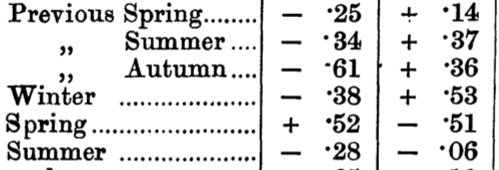
\includegraphics[width=0.8\linewidth]{images/Hooker-correlations}

Now to quote from the recollections published in 1908 by \href{https://en.wikipedia.org/wiki/William_Sealy_Gosset}{William Seely Gossett}, writing anonymously as ``Student'':

\begin{quote}
\emph{Dr Shaw made an enquiry as to the significance of correlation coefficients derived fronm small numbers of cases.}
\end{quote}

The small number here is 21: Hooker had worked with 21 years of crop and weather data. The plain meaning of ``significance of'' here is ``the meaning carried by.'' A modern person might have asked, ``Some of those correlations are pretty small. And you don't have much data. Do such small correlations mean anything?'' To continue \ldots{}

\begin{quote}
\emph{His question was answered by Messrs \href{https://en.wikipedia.org/wiki/Udny_Yule}{Yule} and \href{https://en.wikipedia.org/wiki/Reginald_Hawthorn_Hooker}{Hooker} and Professor \href{https://en.wikipedia.org/wiki/Francis_Ysidro_Edgeworth}{Edgeworth}, all of whom considered that Mr Hooker was probably safe in taking .50 as his limit of significance for a sarnple of 21.}
\end{quote}

In plainer language: don't take as meaningful any correlation coefficient less than 0.50.

\begin{quote}
\emph{They did not, however, answer Dr Shaw's question in any more general way. Now Mr Hooker is not the only statistician who is forced to work with very small samples, and until Dr Shaw's question has been properly answered the results of such investigations lack the criterion which would enable us to make full use of them. The present paper, which is an account of some sampling experimiients, has two objects: (1) to throw some light by empirical methods on the problem itself, (2) to endeavour to interest mathematicians who have both time and ability to solve it.}
\end{quote}

A general solution was found, in part by Student but also by others such as Ronald Fisher. Key to setting up the solution was to define ``significance'' in mathematical terms. The setup was logically ingenious and a little hard to follow. It goes like this:

Suppose we have two variables that have been generated entirely at random and independently of one another. We can calculate the correlation coefficient between them. The correlation coefficient will also be a random number, presumably near zero. If we perform the experiment many times and collect the set of random correlation coefficients produced, we will have an idea of what is the size of commonly encountered coefficients, and how big a correlation coefficient should be so that we can sensibly regard it as being unlikely to arise from random, independent variables.

Doing the random-and-independent-variable simulation for the \(n = 21\) situation of Hooker's paper, indicates that a correlation coefficient at or above 0.50 will result about 1\% of the time. That's a small probability. So, as Messrs Yule, Hooker, and Edgeworth said, it seems ``pretty safe'' -- 99\%? -- to conclude that \(r = 0.50\) with \(n=21\) means that there \emph{is} an association between the two variables.

Actually, the simulation only tells us about a hypothetical world -- called the \emph{Null Hypothesis} -- in which variables are random and independent. The simulation doesn't have anything to say about a world in which variables are related to one another. It's legitimate to say that observing something that's very unlikely -- 1\% chance of \(r \ge 0.5\) -- suggests that the data didn't come from that world. But suppose data came from another hypothetical world -- called the \emph{Alternative Hypothesis} -- where variables are related to one another. Such a world might easily generate a value \(r < 0.5\). So seeing large r entitles us to ``reject the null hypothesis,'' but seeing small r doesn't tell us about the alternative hypothesis. Small r just means that we can't reject the null hypothesis. The formal language is ``fail to reject the null hypothesis.''

The probability that comes from the null hypothesis simulation has a name: the \emph{p-value}.

In 1925, Ronald Fisher suggested using a probability of 5\% instead of 1\% in lab work. This guideline was intended to help lab workers avoid making unwarranted claims that an experiment is showing a positive result. If the p-value is \(p > 0.05\), you have nothing to say about your experiment, you \emph{fail to} reject the null hypothesis.

Over the years, this got turned around. When \(p < 0.05\) (by convention), you're entitled to ``reject the null hypothesis.'' In order to publish a scientific report, researchers were obliged to have enough data to reject the null. This is a way of saying that \emph{some} non-null claim is warranted. But which ones? Certainly the point is to show that there is some substantial relationship between the response and explanatory variable(s), a relationship that means something in the real world. Rejecting the null is not, on its own, a sign that the relationship is substantial and meaningful.

Further confusing things was that little word used by Dr Shaw in 1907: \emph{significance}. An equivalence developed between ``reject the null'' and ``significance.'' Claims that had a low p-value came to be described as ``statistically significant.'' In everyday speech, ``significant'' means substantial or meaningful or important. This is \emph{not} the meaning of ``statistically significant.'' The importance or meaning of an association between a response and explanatory variables can be assessed by looking at the \emph{effect size}, and checking whether the effect size is large enough to have practical meaning in the world. But even tiny effect sizes, without any practical implications, can generate small p-values. You just have to have enough data. With the phrase ``statistically significant'' attached to findings, people could publish their work even if there was no practical meaning.

It's worse than this. Even when variables are unrelated, the p-value will be smaller than 0.05 on five percent of occasions. When Fisher was writing in 1925, there weren't many researchers and each lab experiment required a lot of work. And, in any event, ``rejecting the null'' was just an internal check on what lab work is worth following up and replicating. But today there are millions of researchers. And each researcher can easily look at dozens of variables. So, even if every researcher was working with unrelated variables, statistical significance will be found millions of times: enough to saturate the literature and effectively hide genuine findings with practical significance.

After decades of researchers mis-using p-values, in 2019 the American Statistical Association, a leading professional organization world-wide, issued a statement worth quoting in length:

\begin{quote}
It is time to stop using the term 'statistically significant" entirely. Nor should variants such as ``significantly different,'' ``p \textless{} 0.05,'' and ``nonsignificant'' survive, whether expressed in words, by asterisks in a table, or in some other way.

Regardless of whether it was ever useful, a declaration of ``statistical significance'' has today become meaningless. Made broadly known by Fisher's use of the phrase (1925), Edgeworth's (1885) original intention for statistical significance was simply as a tool to indicate when a result warrants further scrutiny. But that idea has been irretrievably lost. Statistical significance was never meant to imply scientific importance, and the confusion of the two was decried soon after its widespread use (Boring 1919). Yet a full century later the confusion persists.

And so the tool has become the tyrant. The problem is not simply use of the word ``significant,'' although the statistical and ordinary language meanings of the word are indeed now hopelessly confused (Ghose 2013); the term should be avoided for that reason alone. The problem is a larger one, however: using bright-line rules for justifying scientific claims or conclusions can lead to erroneous beliefs and poor decision making (ASA statement, Principle 3). A label of statistical significance adds nothing to what is already conveyed by the value of p; in fact, this dichotomization of p-values makes matters worse.

For example, no p-value can reveal the plausibility, presence, truth, or importance of an association or effect. Therefore, a label of statistical significance does not mean or imply that an association or effect is highly probable, real, true, or important. Nor does a label of statistical nonsignificance lead to the association or effect being improbable, absent, false, or unimportant. Yet the dichotomization into ``significant'' and ``not significant'' is taken as an imprimatur of authority on these characteristics. In a world without bright lines, on the other hand, it becomes untenable to assert dramatic differences in interpretation from inconsequential differences in estimates. As Gelman and Stern (2006) famously observed, the difference between ``significant'' and ``not significant'' is not itself statistically significant.

Furthermore, this false split into ``worthy'' and ``unworthy'' results leads to the selective reporting and publishing of results based on their statistical significance---the so-called ``file drawer problem'' (Rosenthal 1979). And the dichotomized reporting problem extends beyond just publication, notes Amrhein, Trafimow, and Greenland (2019): when authors use p-value thresholds to select which findings to discuss in their papers, ``their conclusions and what is reported in subsequent news and reviews will be biased\ldots{}Such selective attention based on study outcomes will therefore not only distort the literature but will slant published descriptions of study results---biasing the summary descriptions reported to practicing professionals and the general public.'' For the integrity of scientific publishing and research dissemination, therefore, whether a p-value passes any arbitrary threshold should not be considered at all when deciding which results to present or highlight.
\end{quote}

\hypertarget{appendix-when-df-geq-2}{%
\section{\texorpdfstring{Appendix: When \(df \geq 2\)}{Appendix: When df \textbackslash{}geq 2}}\label{appendix-when-df-geq-2}}

For models with multiple explanatory variables or categorical variables with more than two levels, the critical values of F differ substantially from the \(df = 1\) case only for very small \(n\).

\begin{longtable}[]{@{}llllllllll@{}}
\toprule
Sample size \(n\) & large & 10 & 9 & 8 & 7 & 6 & 5 & 4 & 3\tabularnewline
\midrule
\endhead
\(df = 1\) & 4 & 5 & 5.3 & 5.6 & 6 & 7 & 8 & 10 & 19\tabularnewline
\(df = 2\) & 3 & 4.5 & 4.7 & 5.1 & 5.7 & 7 & 9.5 & 19 & 200\tabularnewline
\(df = 3\) & 2.7 & 4.3 & 4.8 & 5.4 & 6.6 & 9.3 & 19 & 216 & NA\tabularnewline
\(df = 4\) & 2.5 & 4.5 & 5.2 & 6.4 & 9.1 & 19 & 225 & NA & NA\tabularnewline
\bottomrule
\end{longtable}

\emph{Figure 3: Critical values for F for small \(n\) and a few different values of \(df\).}

\hypertarget{simple-means-and-proportions}{%
\chapter{Simple means and proportions}\label{simple-means-and-proportions}}

The presentation of classical inferene in this compact guide does not follow the historical flow of how inferential concepts were developed, largely over the half century from 1880 to 1925. Instead we started with F, which dates from 1925, introducing it in the context of models, an even more recent concept. Models provide a means to address contemporary uses of data.

Historically, inference started with very simple questions involving a single variable. For instance, after observing a mental-health patient's sleep over several days, a reasonable presentation of how much sleep the patient got is the the mean over those days. Or, in a more contemporary context, imagine being interested in the trend toward self-driving cars. A reasonable summary of the deployment of the technology could be the proportion of cars on the road with self-driving features such as lane-keeping or automatic braking before a collision.

Very often, behind the interest in a mean or proportion is a different interest: a change in mean or a change in proportion. For such questions, models and F are the way to go. But in this chapter we'll journey into neans and proportions themselves.

\hypertarget{no-flexibility-df-0}{%
\section{No flexibility: df = 0}\label{no-flexibility-df-0}}

We seen that models can be constructed with more or less flexibility, e.g.~more or fewer explanatory variables, more or fewer levels in a categorical variable. It is possible to think about a simple mean or a simple proportion in terms of a model, but it is a strange model with \emph{no explanatory variables}. That is, it is a model with \(df = 0\).

Consider the general formula for F:

\[ \mbox{F} \equiv \frac{n - (1+df)}{df} \frac{v_m}{v_r - v_m}\]

Since F involves division by \(df\), the ratio is indeterminate. Or, in the words of your third-grade teacher, ``You're not allowed to divide by zero.''

But \(df=0\) is not the only thing going on when doing inference on a mean or proportion. The model itself is unusual. Because there is no explanatory variable, the model has no input. A function with no input can, mathematically, have only one value for the output. And so the model values will always be the same. This implies \(v_m = 0\). As for the effect size of the model, there's no changing output and no input to change, so the usual definition of change-in-output / change-in-input doesn't apply.

In the spirit of discussion (as opposed to mathematical proof), let's imagine filling in the values \(df=0\) and \(v_m=0\) into the formula for F and let's take the effect size B to be the (constant) model output itself. For F we get

\[\mbox{F}  = \frac{n - 1}{0} \frac{0}{v_r} \approx \frac{n-1}{v_r}\ \ \ \ \mbox{WARNING: Cancelling out zeros is not legit.}\]

Using that F, and ignoring its illegitimate derivation, we can find the CI with the usual CI formula,

\[CI = B (1 \pm \sqrt{4/\mbox{F}}) = B (1 \pm 2 \sqrt{n-1} / s_r).\]
What's \(s_r\). It's simply \(s_r \equiv \sqrt{v_r}\).

It turns out that this expression for CI, however sketchy the means of arriving at it, is correct. We got to the right answer by making two mistakes that cancelled out.

In classical inference, the quantity

\[\mbox{SE} = \frac{s_r}{\sqrt{n-1}}\]

has a name: the standard error (SE) of the mean. And \(s_r\) itself has a name: the standard deviation of the (response) variable.

When it comes to interpreting the F value itself, the mistakes we made don't cancel out. The correct value for F is

\[\mbox{F} \equiv (B / \mbox{SE})^2 = (n-1) \frac{B^2}{v_r}\]

This quantity was invented decades before F was introduced to statistics. Strictly speaking, the quantity that was invented is the square root of the above and it is given the name \emph{t}:

\[\mbox{t}  = B / SE.\]

Hypothesis tests that were based on t were called ``t-tests,'' a name that will be familiar to anyone who took a conventional statistics course.

\hypertarget{covariates}{%
\chapter{Covariates}\label{covariates}}

\hypertarget{comparing-models}{%
\chapter{Comparing models}\label{comparing-models}}

Looking at \(\Delta F\).

\hypertarget{outside-the-normal-situation}{%
\chapter{Outside the normal situation}\label{outside-the-normal-situation}}

About ranks, transformations, \ldots{}

\hypertarget{remember-inference-isnt-everything}{%
\chapter{Remember, inference isn't everything}\label{remember-inference-isnt-everything}}

Study design, sampling bias, etc.

\bibliography{book.bib}


\end{document}
